\mnAdvanced\PID 
Отпорност отпорника чија је толеранција $5\%$ представља 
насумичну променљиву 
функције расподеле густине вероватноће, 
која се може сматрати да је униформна, у опсегу $\pm5{\%}$ своје средње вредности $R_0$. 
(а) Одредити функцију расподеле густине вероватноће отпорности два таква редно везана отпорника, отпорности 
$R_0 = 1\unit{k\Omega}$. 
(б) Упоредити добијену расподелу са расподелом једног отпорника отпорности $2R_0 = 2\unit{k\Omega}$.    
\vspace*{2mm}

\textsc{\underline{Решење:}}
Функција расподеле густине вероватноће једног отпорника је дата изразом $p(R) = \rect\left(\dfrac{R - R_0}{0,1\, R_0}\right)$. 
Отпорност редне везе једнака је збиру појединачних отпорности $R = R_1 + R_2$. Да бисмо одредити функцију расподеле 
густине ове вероватноће запишимо то као $R = r + \underbrace{(R - r)}_{R_2}$, где је $r$ једна реализација отпорности 
првог отпорника. Одатле за густину вероватноће збира важи 
\begin{equation}
\de p_{\Sigma}(R) = 
\underbrace{p(r) \de r}_{\text{Први отпорник}}
\cdot \underbrace{p(R - r) \de r}_{\text{Други отпорник}},
\end{equation} при чему се вероватноће множе јер су то међусобно независни догађаји.
Даље се дељењем обе стране са $\de r$ па потом интеграцијом по $r$ налази:
\begin{equation}
    \dfrac{\de p_{\Sigma}(R)}{\de R} = 
    p(r) 
    \cdot p(R - r) \de r 
    \Rightarrow
    p_{\Sigma}(R) = \underbrace{\int_{-\infty}^{\infty} p(r) \cdot p(R - r) \de R}_{\text{Конволуциони интеграл}},
\end{equation}
где идентификујемо \textit{конволуциони интеграл} па се овај резултат може записати и као
$p_{\Sigma}(R) = p(R) \ast p(R)$.

Сада функцију густине вероватноће можемо одредити применом особина конволуције. 
Приметимо да је $p(R) = \dfrac{1}{0,1 R_0} \rect\left(\dfrac{R - R_0}{0,1\, R_0}\right) = 
\rect\left(\dfrac{R}{0,1 R_0}\right) \ast \updelta(R - R_0)$, па се даље има
\begin{align}
    p_{\Sigma}(R) =& 
    \underbrace{
    \dfrac{1}{0,1 R_0} \rect\left(\dfrac{R}{0,1 R_0}\right) \ast \updelta(R - R_0)
    }_{p(R)}
    \ast 
    \underbrace{
    \dfrac{1}{0,1 R_0} \rect\left(\dfrac{R}{0,1 R_0}\right) \ast \updelta(R - R_0) 
    }_{p(R)}
    \\
    =&
    \left(\dfrac{1}{0,1 R_0}\right)^2 \rect\left(\dfrac{R}{0,1 R_0}\right) \ast \rect\left(\dfrac{R}{0,1 R_0}\right) 
    \ast \underbrace{\updelta(R - R_0) \ast \updelta(R - R_0)}_{\updelta(R - 2R_0)},
    \\
    =&  \left(\dfrac{1}{0,1 R_0}\right) \tri\left( \dfrac{R}{0,1 R_0} \right) \ast \updelta(R - 2R_0) 
    =  \left(\dfrac{1}{0,1 R_0}\right) \tri\left( \dfrac{R - 2R_0}{0,1 R_0} \right) 
\end{align}
пре чему је у првом кораку употребљена асоцијативност конволуције а у другом 
је примењено својство скалирања аргумента 
$x(t) \ast x(t) = y(t) \Rightarrow x(kt) \ast x(kt) = \dfrac{1}{k} y(kt)$, уз табличну 
трансформацију\footnote{Видети и таблицу \reft{T:ctc:rect}} $\rect(t) \ast \rect(t) = \tri(t)$. 

(б) Тражено поређење је приказано на слици \ref{fig:\ID}.

\begin{figure}[ht!]
    \centering
    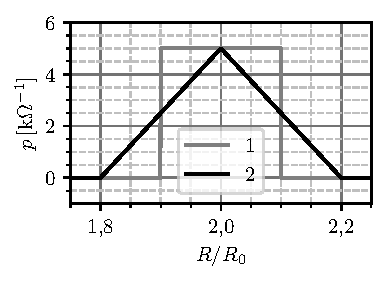
\includegraphics{fig/probabilities.pdf}
    \caption{
        Расподела густине вероватноће за: 1 -- један отпорник отпорности $2\unit{k\Omega}$; и
        2 -- редну везу два отпорника отпорности $1\unit{k\Omega}$.
    }
    \label{fig:\ID}

\end{figure}